\documentclass{beamer}

\usepackage{graphicx}

% Informacion
\title{Computer Graphics in the 60s}
\author{
  Liang, Binjie | \texttt{2023064642} \\
  \and
  Apellidos, Nombre | \texttt{carnet} \\
  \and
  Apellidos, Nombre | \texttt{carnet} \\
  \and
  Apellidos, Nombre | \texttt{carnet} \\
}
\institute{Campus Tecnológico Local San José}
\date{2026 | II Semester}

\begin{document}

% se define portada (no tocar)
\frame{\titlepage}


\begin{frame}
\frametitle{Introduction of CG Term}

\begin{columns}

    % Image on the left
    \begin{column}{0.48\textwidth}
        \centering
        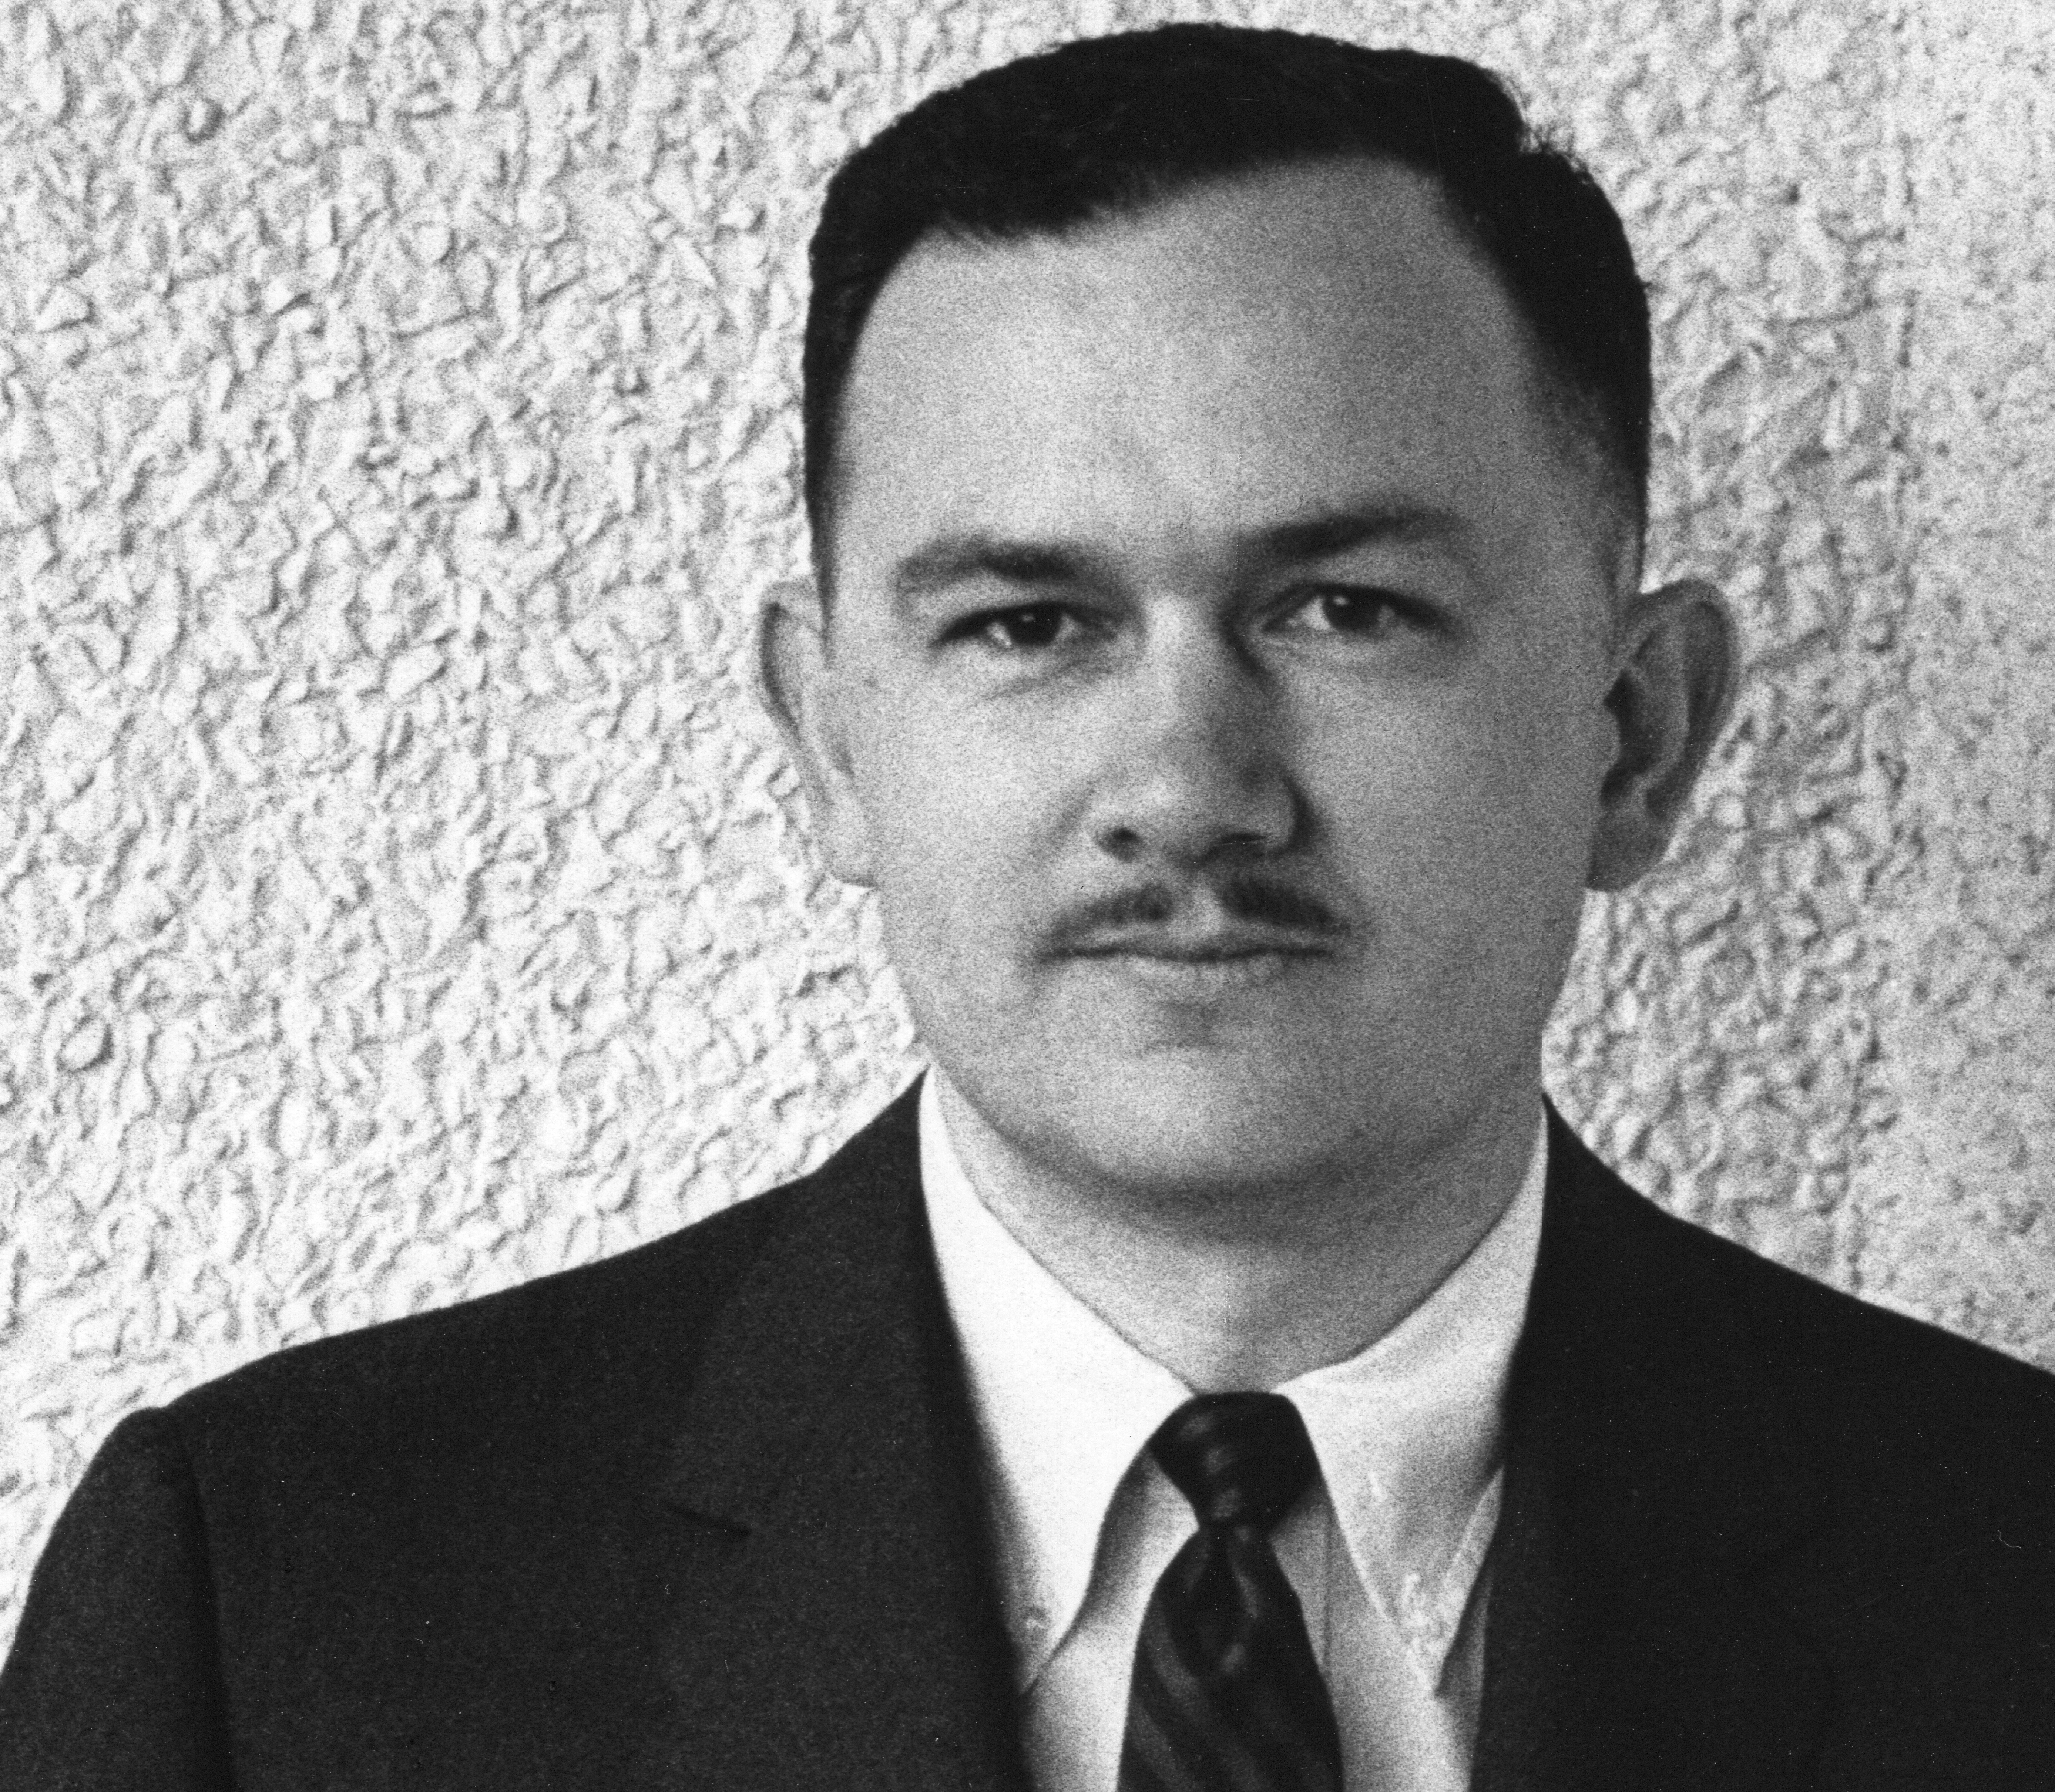
\includegraphics[width=\linewidth]{assets/WilliamFetter.jpg}
    \end{column}

    % Text on the right
    \begin{column}{0.48\textwidth}
        William A. Fetter coined the CG term while he was working as a graphics designer at Boeing in 1960.
    \end{column}

\end{columns}

\end{frame}
%==================================================================================
\begin{frame}
\frametitle{First Boeing Man}

He was the first person to represent the human figure as a 3D model.
He created the model to study ergonomics and pilot visibility in aircraft cockpits.

\vspace{0.5cm}

\begin{columns}

    \begin{column}{0.48\textwidth}
        \centering
        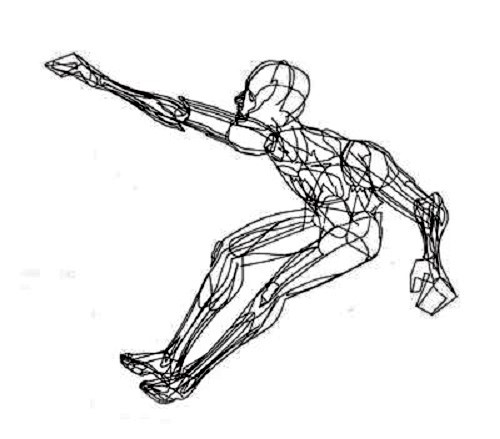
\includegraphics[width=\linewidth]{assets/BoeingMan.jpg}
        
        \small First Boeing Man 
    \end{column}

    \begin{column}{0.48\textwidth}
        \centering
        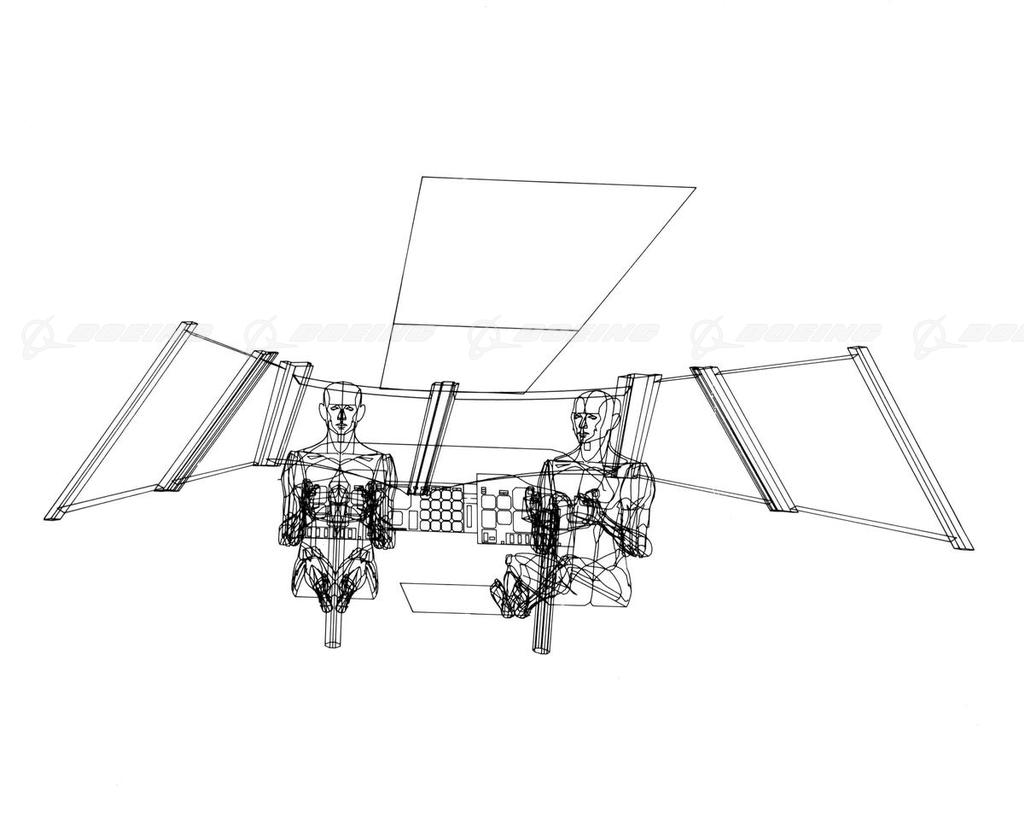
\includegraphics[width=\linewidth]{assets/pilots.jpg}
        
        \small Pilots visibility in cockpit
    \end{column}

\end{columns}

\end{frame}
%==================================================================================

\begin{frame}
\frametitle{1961 - Spacewar by Steven Russell}

\begin{columns}

    % Image on the left
    \begin{column}{0.48\textwidth}
        \centering
        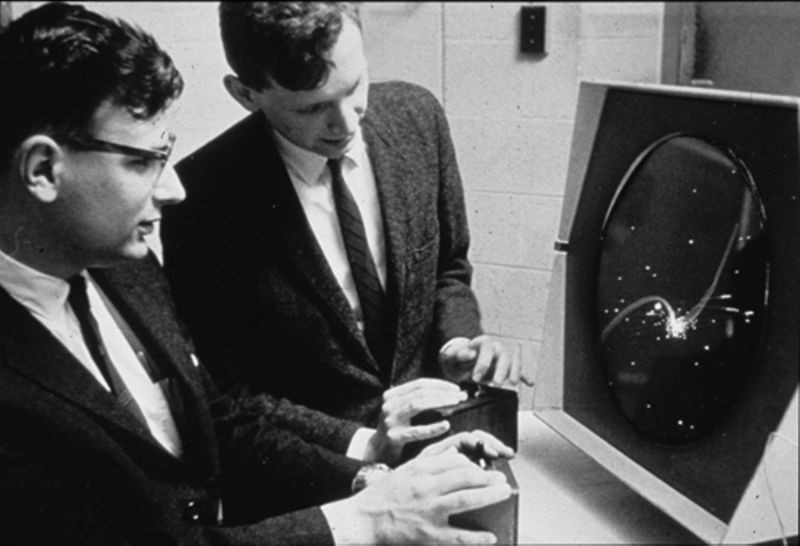
\includegraphics[width=\linewidth]{assets/spacewar.jpg}
    \end{column}

    % Text on the right
    \begin{column}{0.48\textwidth}
        In 1961, the MIT student Steven Russell developed Spacewar game. It was the first video game for the DEG PDP-1 minicomputer in 1962, this computer is important since it was the first commercial computer centered in direct user interaction. Thanks to the PDP-1, the hacker culture in the MIT rose.
    \end{column}

\end{columns}

\end{frame}

% ====================================================================================

\begin{frame}
\frametitle{1963 - Sketchpad by Ivan Sutherland}

\begin{columns}

    % Image on the left
    \begin{column}{0.48\textwidth}
        \centering
        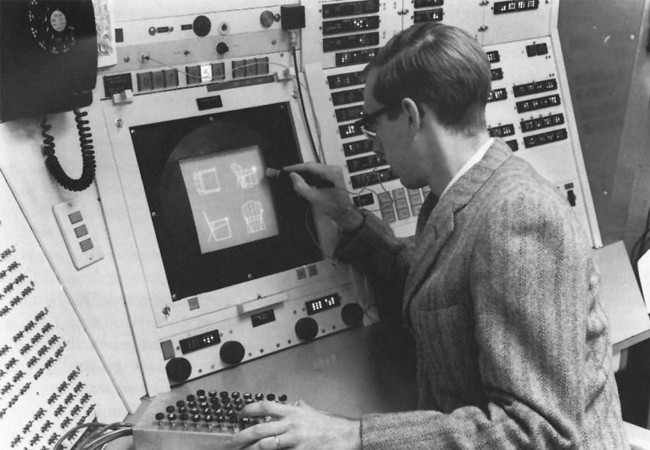
\includegraphics[width=\linewidth]{assets/sketchpad.jpg}
    \end{column}

    % Text on the right
    \begin{column}{0.48\textwidth}
        In 1963, Ivan Sutherland developed the Sketchpad for his doctoral thesis at MIT. This is important, since it was the first time that users could use a light-pen to draw shapes on a vector-based monitor. 
        Sutherland also introduced the concept of pop-up menus.
    \end{column}

\end{columns}

\end{frame}

% ====================================================================================

\begin{frame}
\frametitle{1963 - The Mouse by Doug Engelbart}

\begin{columns}

    % Image on the left
    \begin{column}{0.48\textwidth}
        \centering
        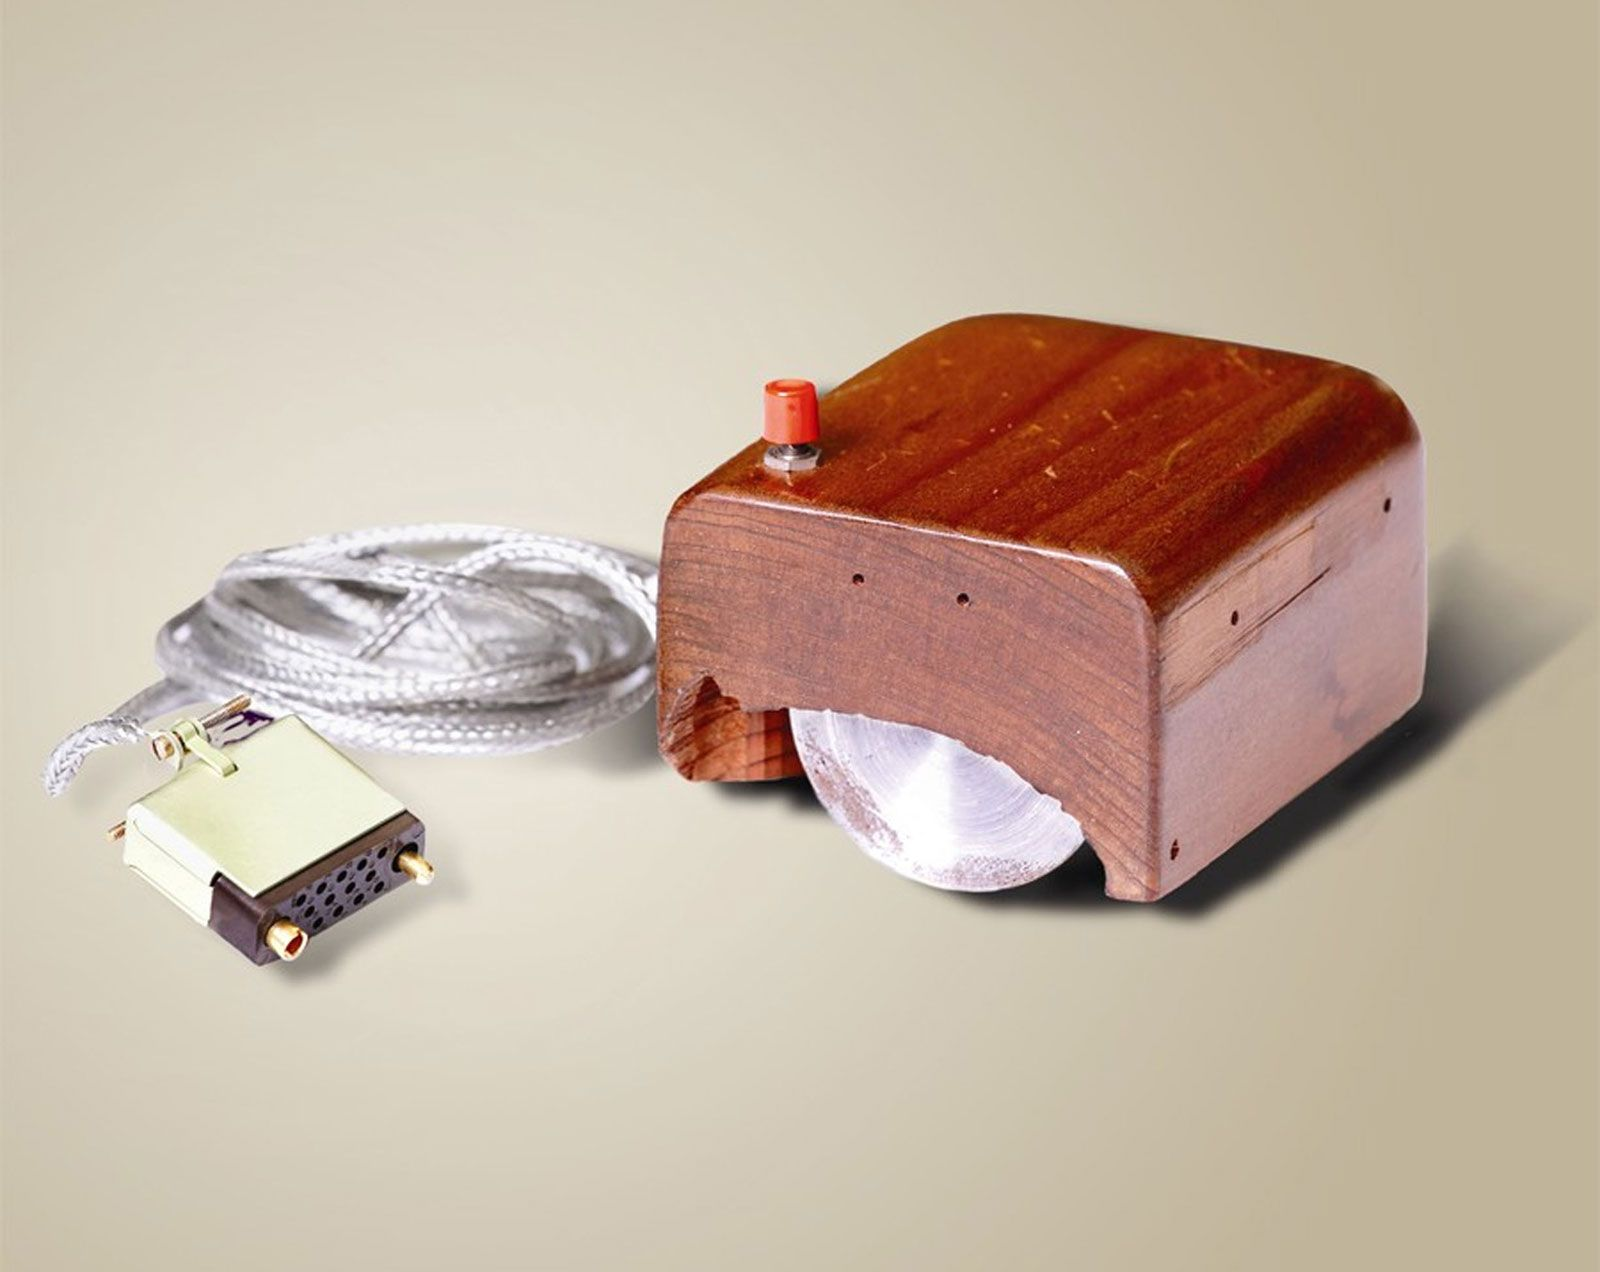
\includegraphics[width=\linewidth]{assets/mouse.jpg}
    \end{column}

    % Text on the right
    \begin{column}{0.48\textwidth}
        In 1963, Doug Engelbart invented the mouse at the Stanford Research Institute. The first prototype was made of a wooden shell, two wheels to track X-Y movements and a circuit-board.
    \end{column}

\end{columns}

\end{frame}

% ====================================================================================

\begin{frame}
\frametitle{1963 - The Hidden-Line Removal by Larry Roberts}

\begin{columns}

    % Image on the left
    \begin{column}{0.48\textwidth}
        \centering
        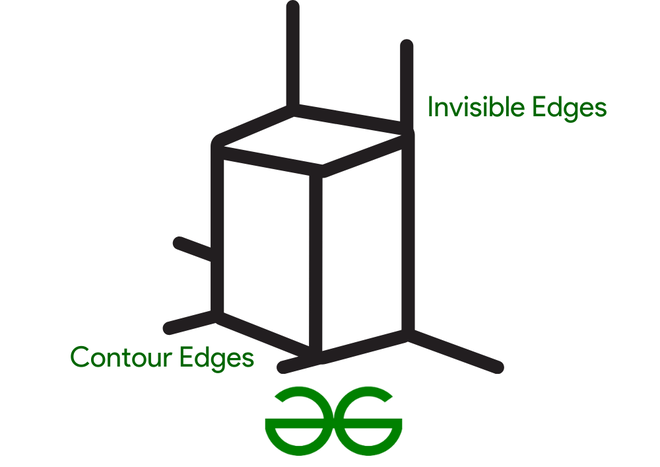
\includegraphics[width=\linewidth]{assets/hidden-line.png}
    \end{column}

    % Text on the right
    \begin{column}{0.48\textwidth}
        Contributing more to the 60s, Larry Roberts developed the first effective hidden-line removal algorithm. In simple words, it was an algorithm that removes the lines that should hidden in what it was supposed to be a 3D object. This algorithm helped to developed 3D objects rendering accurately.
    \end{column}

\end{columns}

\end{frame}

\end{document}
